\documentclass{article}
\usepackage{graphicx}
\usepackage{booktabs}
\usepackage{amsmath}
\usepackage{caption}
\usepackage[margin=1in]{geometry}
\usepackage[section]{placeins}
\usepackage{float}

\captionsetup{font=small}

\title{Multi-Sleeve Statistical Arbitrage Portfolio Construction for U.S. Equities}
\author{Joseph Platta}
\date{May 2026}

\begin{document}

\maketitle

\section{Introduction}

This report documents the construction and evaluation of a diversified multi-sleeve statistical arbitrage portfolio in U.S. equities. The final portfolio combines six distinct signal families (momentum, active return mean reversion, residual return mean reversion, distance-pairs relative value, sector-relative mean reversion, and event-driven gap reversion) into a single dollar-neutral long-short portfolio. The research followed a multi-step process that begins with a broad search across multiple alpha families. Next, conditioning and risk scaling are used to improve regime robustness. Portfolio construction begins by paring uncorrelated signals into equal weighted portfolios. The final portfolio is constructed using stability verification through ablation tests and alternative weighting schemes.

The final portfolio achieves an in-sample net Sharpe ratio greater than 2.0 after 10 basis points of assumed transaction costs during the 2015--2023 period. During the out-of-sample period (2024--2026), performance degrades, but remains profitable while preserving much of the portfolio's diversification structure. The results suggest that diversification across heterogeneous mean reversion and momentum sleeves might produce more stable portfolio level behavior than reliance on any single standalone signal. Several sleeves with moderate standalone performance contribute meaningfully through low cross correlation and complementary regime specialization.

\section{Methodology \& Experimental Setup}

All data is sourced from yfinance daily close prices. The portfiol is built using S\&P 500 equities as the univsere. This universe is filtered to the 300 most liquid names at any given time, where liquidity is defined as 60-day rolling average dollar volume (price $\times$ daily shares traded) ranked cross-sectionally each day. The SPY ETF is used as a benchmark. The factor set used in the study uses SPY as the market factor and then relies on the following sector ETFs as factors: XLK, XLF, XLE, XLV, XLI, XLY, XLP, XLU, XLRE, XLB. The signals and portfolio is developed against an in-simple period 2015--2013 and the final portfolio is evaluated against the out-of-sample period January 2024 through April 2026.

The following assumptions are made throughout the research process. Portfolio construction uses a dollar-neutral long-short approach consisting of 20 long and 20 short positions with equal weighting applied within each sleeve. Signals are processed using a cross-sectional rank transformation and shifted forward by one trading day to eliminate lookahead bias. Portfolios are rebalanced at fixed deterministic intervals of 1, 5, 10, or 21 trading days depending on the underlying signal horizon. Transaction costs are modeled as a constant linear cost of 10 basis points per trade with no additional assumptions for market impact or slippage. The strategy remains fully invested at all times while risk exposure is dynamically scaled using an equity-curve regime filter: when a strategy's equity curve falls below its 20 day moving average, then portfolio exposure is reduced to 25\% of nominal size.

The multi-step research process moves from broad signal discovery toward increasingly structured portfolio construction and robustness testing. The first step focused on identifying promising sources of cross-sectional alpha across several distinct strategy families including momentum, multiple forms of mean reversion, distance-pairs trading, sector-relative dislocations, and event-driven gap effects. Multiple versions of each signal are systematically explored using different return definitions, lookback windows, and rebalance frequencies. The focus at this step is deliberately exploratory rather than optimization. The aim is to identify signal families exhibiting persistent predictive structure without relying on aggressive conditioning or parameter tuning.

The strongest standalone signals are rebuilt with regime aware conditioning and some dynamic risk scaling overlays. The conditioning filters are used as gating mechanisms to selectively enable or disable exposure under specific market environments. The gating mechanisms explored include trend, volatility, breadth, correlation, dispersion, panic, and sector dislocation regimes. All sleeves also incorporated a baseline equity curve risk scaler that reduced exposure when a strategy's recent performance deteriorated. After conditioning, the return correlations of the best performing sleeves are explored and used to combine complementary signals into pairwise portfolios. This step identifies which sleeves contributed genuinely additive diversification benefits versus those that were largely redundant.

The final steps focus on higher level portfolio architecture and robustness. Using insights from the pairwise interaction analysis, several hand designed target portfolios are constructed around distinct investment philosophies: conservative low turnover designs to more aggressive volatility sensitive structures. The best configuration intentionally combines defensive mean reversion sleeves with more aggressive distance-pairs and volatility expansion sleeves to balance stability and convexity across market regimes. These portfolios are further extended with additional momentum, event-driven, and sector-relative sleeves under multiple weighting schemes including equal weight, volatility scaled, Sharpe scaled, and ridge regularized mean variance optimization. Finally, ablation testing removes some individual sleeves and entire strategy families to verify that portfolio performance isn't dependent on any single sleeve and that the diversification structure remains stable.

\section{Signals}

All signals are tested as dollar-neutral cross-sectional portfolios, with ranking, rebalancing, liquidity constraints, and transaction cost assumptions applied consistently across all experiments. Six different signal families are explored: momentum, active return mean reversion, residual return mean reversion, sector-relative mean reversion, distance-pairs mean reversion, and gap reversion.

\begin{table}[H]
    \centering
    \small
    \begin{tabular}{llrrr}
        \toprule
        Family & Variant & Net Sharpe & Turnover & Max DD \\
        \midrule
        \textbf{Monotonic Momentum} & Base (120d, rebal 21d) & 0.606 & 5.100\% & $-$14.700\% \\
        & + low-dispersion scaling (60d, q30) & 0.769 & 3.983\% & $-$10.146\% \\
        \midrule
        \textbf{Active-Return MR} & Base (5d reversal, rebal 10d) & 0.557 & 11.700\% & $-$12.900\% \\
        & + uptrend scaling (20/100d) & 0.708 & 5.200\% & $-$6.700\% \\
        & + high residual dispersion gate (20d, q75) & 1.279 & 1.733\% & $-$3.173\% \\
        \midrule
        \textbf{Residual MR} & Base (ETF-factor 5d, rebal 10d) & 0.694 & 11.900\% & $-$7.900\% \\
        & + uptrend scaling (20/100d) & 0.918 & 5.100\% & $-$4.400\% \\
        & + high residual dispersion gate (20d, q75) & 1.083 & 1.542\% & $-$4.538\% \\
        \midrule
        \textbf{Distance-Pairs MR} & Base ($k$=3, 60d z-score, rebal 10d) & 1.078 & 12.911\% & $-$9.709\% \\
        \midrule
        \textbf{Sector-Relative} & Base (z-score 5/60, rebal 10d) & 0.248 & 11.900\% & $-$15.200\% \\
        & + uptrend scaling (20/100d) & 0.584 & 5.100\% & $-$5.000\% \\
        & + high residual dispersion gate (20d, q75) & 0.886 & 2.021\% & $-$5.926\% \\
        \midrule
        \textbf{Event / Gap Reversion} & Base (residual gap reversal, rebal 10d) & 0.626 & 11.100\% & $-$10.500\% \\
        & + uptrend scaling (50/200d) + vol contraction gate & 0.825 & 3.599\% & $-$4.383\% \\
        \bottomrule
    \end{tabular}
    \caption{Signal conditioning progression from base through best risk-scaled and conditioned variants. Monotonic Momentum and Distance-Pairs MR showed no improvement from conditioning beyond the rows shown.}
    \label{tab:conditioning-progression}
\end{table}

Table 1 shows the progression from base (no scaling, no conditioning) through the best risk scaled variant to the best conditioned variant for each family. This illustrates how much of the final signal quality came from the raw signal versus the overlay.

The largest improvements came from conditioning in the active return mean reversion and sector-relative families. For these families the gating to high residual-dispersion regimes more than doubled the net Sharpe while cutting turnover by roughly 80\%. For distance-pairs, neither scaling nor conditioning improved the base signal. The raw relative-value convergence signal is already strong on its own. For monotonic momentum, dispersion scaling helped but conditioning added nothing further.

The consistent pattern across families: conditioning filters improved net Sharpe primarily by reducing turnover (and therefore cost drag) rather than by increasing gross alpha. The filters act as regime gates that keep the strategy out of environments where its signal is noisy rather than amplifying the signal in good environments.

Several patterns stand out across families. The conditioned mean reversion variants --- both active-return and residual --- achieved the highest net Sharpes when gated to high residual-dispersion regimes, where cross-sectional idiosyncratic movement is elevated and the reversal signal has more to work with. Distance-pairs mean reversion had the highest gross Sharpe (1.549) but also the highest turnover, making it the most cost-sensitive family. The momentum signal was the only one with meaningful positive benchmark correlation (+0.253), while distance-pairs was the only signal with negative benchmark correlation ($-$0.179) --- making them natural portfolio complements. Sector-relative and event sleeves had near-zero benchmark correlation, meaning they contribute diversification from the index without taking a strong directional view on market regime.

\begin{table}[H]
    \centering
    \resizebox{\textwidth}{!}{%
    \begin{tabular}{llllrrrrr}
        \toprule
        Family & Signal & Scaling & Cond.\ Gate & Net SR & Gross SR & Turnover & Max DD & $\rho_{\text{bench}}$ \\
        \midrule
        Monotonic Mom. & 120d, rebal 21d & Low-disp. & None & 0.769 & 0.910 & 3.983\% & $-$10.146\% & 0.253 \\
        Active-Ret.\ MR & Z-score 5d/60d, rebal 10d & Uptrend 20/100d & High resid.\ disp. & 1.279 & 1.426 & 1.733\% & $-$3.173\% & 0.143 \\
        Residual MR & Factor-model 5d, rebal 10d & Uptrend 20/100d & High resid.\ disp. & 1.083 & 1.192 & 1.542\% & $-$4.538\% & 0.092 \\
        Dist.-Pairs MR & $k$=3, 60d z-score, rebal 10d & None & None & 1.078 & 1.549 & 12.911\% & $-$9.709\% & $-$0.179 \\
        Sector-Rel.\ MR & Sector-rel.\ 5d, rebal 10d & Uptrend 20/100d & High resid.\ disp. & 0.886 & 1.014 & 2.021\% & $-$5.926\% & 0.019 \\
        Event / Gap Rev. & Resid.\ gap rev., rebal 10d & Uptrend 50/200d & Vol contraction & 0.825 & 1.093 & 3.599\% & $-$4.383\% & 0.043 \\
        \bottomrule
    \end{tabular}%
    }
    \caption{Best conditioned signal variant per family.}
    \label{tab:best-conditioned-signals}
\end{table}


\section{Portfolio Construction}

\subsection{Identifying Diversification Opportunities}

Before assembling a portfolio, the return correlations across conditioned sleeves are examined to understand which families might pair well together and why.

\begin{figure}[htbp]
    \centering
    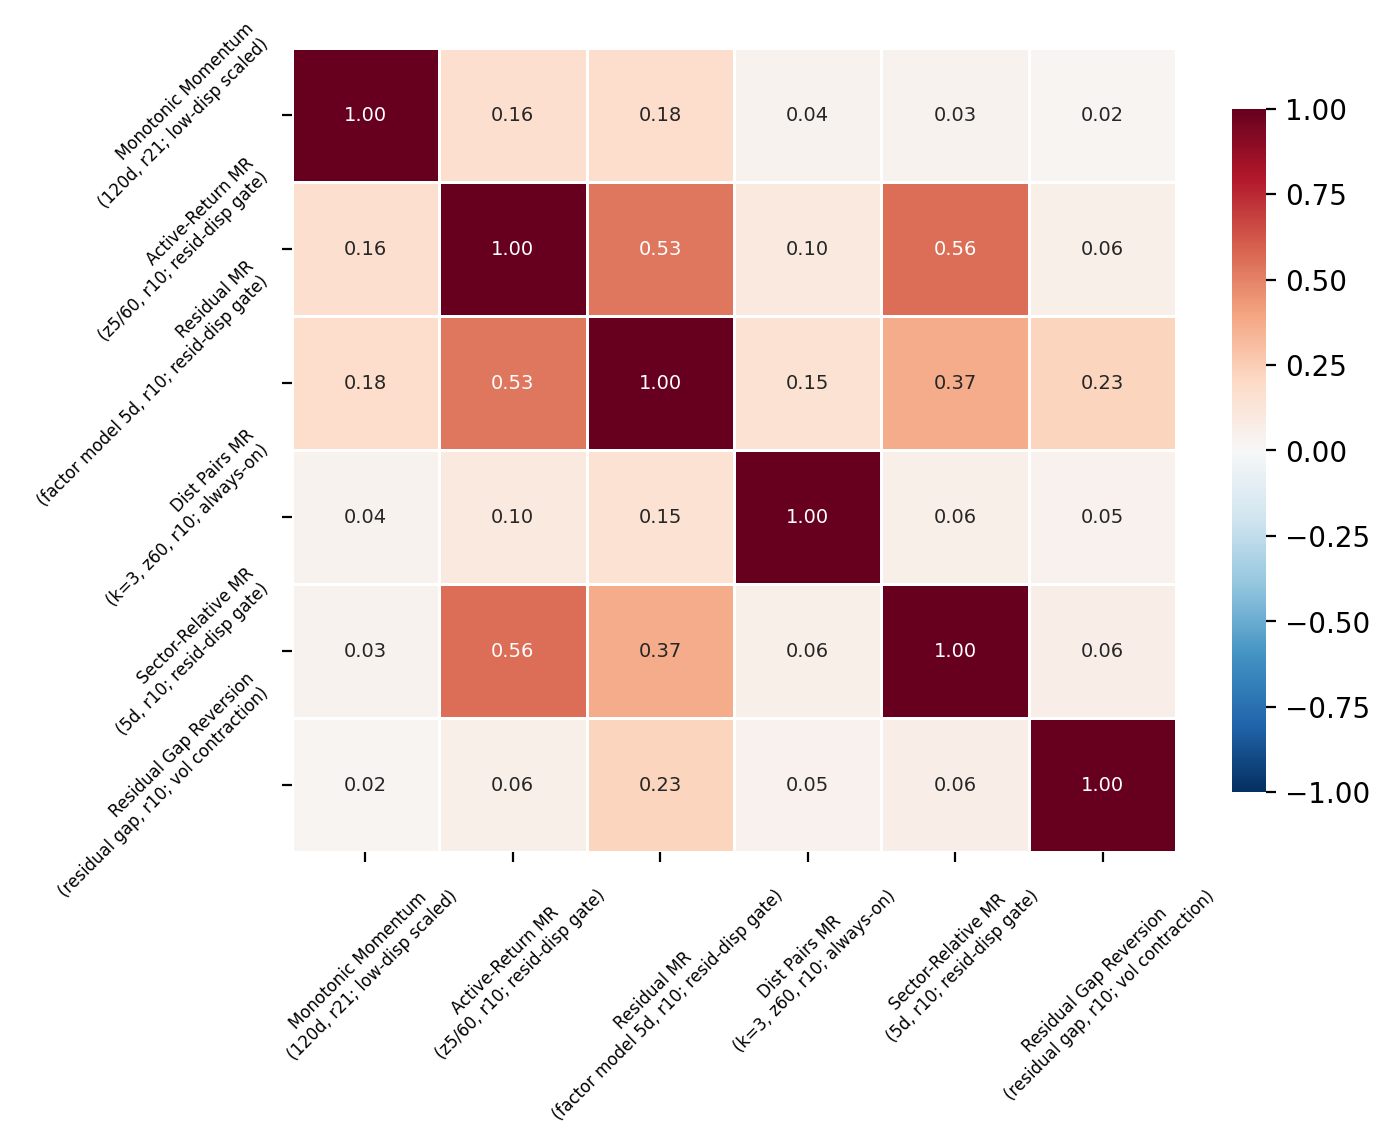
\includegraphics[width=0.75\textwidth]{figures/return_correlations_of_selected_sleeves.png}
    \caption{Return correlations across conditioned sleeves. Two natural groups emerge: a correlated mean-reversion complex and a set of orthogonal diversifiers.}
    \label{fig:correlations}
\end{figure}

The correlation matrix reveals two natural clusters. Active-return MR, residual MR, and sector-relative MR form a correlated block with pairwise correlations in the 0.37--0.56 range. This makes economic sense --- these are all expressions of the same underlying cross-sectional reversal phenomenon. Residualization and sector anchoring change the implementation characteristics and regime behavior, but the core bet is similar: stocks that moved too much recently should revert.

Distance-pairs mean reversion (DPMR) stands apart from this cluster. Its correlations to every other family stay around 0.04--0.15. Even though DPMR is also a form of mean reversion, its reference point is fundamentally different --- it trades convergence toward a stock's nearest historical peers rather than reversal toward a cross-sectional or factor-adjusted mean. That distinction produces a return stream that behaves like a separate alpha source entirely.

Monotonic momentum correlates only 0.16--0.18 with the MR families. This is low enough to suggest that momentum and reversal are structurally complementary rather than offsetting --- a momentum sleeve paired with reversal sleeves should produce genuine diversification rather than cancellation.

Event-driven gap reversion also remains fairly independent, with correlations mostly below 0.23. It captures short-horizon idiosyncratic dislocations on a timescale distinct from both the slower reversal processes and the multi-week momentum signal.

No pair of families exhibits dangerously high correlation. Even the strongest relationship (active-return MR vs sector-relative MR at 0.56) is moderate rather than redundant. This suggests that a multi-engine portfolio combining sleeves across these clusters should produce materially better risk-adjusted performance than selecting any single best signal.

An important finding is that conditioning did not collapse the sleeves into the same regime trade. Despite many sleeves using similar filters (dispersion, breadth, volatility contraction), the realized return streams remained differentiated. Conditioning improved implementation quality without destroying the diversification structure that makes portfolio construction worthwhile.

\subsection{Building the Portfolio}

The correlation analysis points toward a natural portfolio architecture: start with a core of low-correlation sleeves from different families, then layer in additional variants that provide regime-specific exposure. The portfolio is built incrementally, adding one sleeve at a time and tracking the marginal impact on Sharpe and drawdown.

\begin{table}[htbp]
    \centering
    \small
    \begin{tabular}{clcrrrr}
        \toprule
        Step & Sleeve Added & Sleeves & Net SR & Gross SR & Turnover & Max DD \\
        \midrule
        1 & Residual MR (high resid.\ disp.\ gate) & 1 & 1.074 & 1.181 & 1.542\% & $-$4.526\% \\
        2 & + Active-Return MR (breadth gate) & 2 & 1.242 & 1.339 & 1.655\% & $-$6.020\% \\
        3 & + DPMR (z20, vol contraction gate) & 3 & 1.556 & 1.746 & 2.447\% & $-$3.753\% \\
        4 & + DPMR (z60, vol expansion gate) & 4 & 1.720 & 2.031 & 3.799\% & $-$3.105\% \\
        5 & + DPMR (z60, always-on) & 5 & 1.786 & 2.219 & 5.536\% & $-$3.254\% \\
        6 & + DPMR (z10, panic gate) & 6 & 1.883 & 2.297 & 4.699\% & $-$2.811\% \\
        7 & + Monotonic Momentum (crash-gated) & 7 & 1.989 & 2.417 & 4.619\% & $-$3.196\% \\
        8 & + Resid.\ Gap Reversion (breadth-gated) & 8 & 2.039 & 2.548 & 5.020\% & $-$2.347\% \\
        \bottomrule
    \end{tabular}
    \caption{Incremental portfolio buildout. Each row adds one sleeve and reports aggregate statistics.}
    \label{tab:portfolio-buildout}
\end{table}

The buildout starts with two sleeves from the correlated MR cluster: residual MR and active-return MR. These share moderate correlation ($\sim$0.4), so combining them improves Sharpe from 1.07 to 1.24 but does not dramatically reduce drawdown. The real diversification begins at step 3 when the first distance-pairs sleeve is added. Sharpe jumps from 1.24 to 1.56 while max drawdown simultaneously drops from $-$6.0\% to $-$3.8\%. This is the correlation structure from Figure~\ref{fig:correlations} showing up in live portfolio construction --- DPMR's orthogonality to the MR complex translates directly into diversification benefit.

What's unusual is that additional DPMR variants continue adding value even though they belong to the same signal family. All four DPMR sleeves share the same base construction ($k=3$ nearest partners, z-scored spread reversal clipped to $[-2, 2]$), but they differ along three dimensions that make them economically distinct:

\begin{table}[htbp]
    \centering
    \small
    \begin{tabular}{lrcll}
        \toprule
        Sleeve & Z Window & Rebal. & Conditioning & Role \\
        \midrule
        DPMR z10 + panic & 10 & 10d & Panic regime ($-$5\% in 10d) & Fast crisis-reversion; episodic \\
        DPMR z20 + vol contr. & 20 & 21d & Vol contraction (10d $<$ 60d vol) & Slow calmer-market convergence \\
        DPMR z60 + vol exp. & 60 & 5d & Vol expansion (10d $>$ 60d vol) & Persistent dislocation in turbulence \\
        DPMR z60 + none & 60 & 10d & Always on & Baseline structural convergence \\
        \bottomrule
    \end{tabular}
    \caption{Distance-pairs sleeve parametrization. All sleeves share the same base construction ($k=3$ nearest partners, z-scored spread reversal clipped to $[-2, 2]$).}
    \label{tab:dpmr-sleeves}
\end{table}

The conditioning filters effectively partition the same alpha engine across different market environments rather than creating duplicate exposure. The panic sleeve (z10) is the most reactive --- it only trades after severe market drawdowns and has extremely low realized turnover (0.6\% daily) because the condition is rarely active. It functions as an episodic crisis-reversion bet with minimal drag in normal environments. The vol-contraction sleeve (z20) activates during calmer regimes where pair spreads are reverting at a steady pace. The vol-expansion sleeve (z60) captures persistent dislocations in turbulent environments using the fastest rebalance (5d). The always-on sleeve (z60) is the structural convergence engine --- no gate means it trades in all regimes, which makes it the highest-turnover component (12.9\% daily) but also the highest standalone Sharpe (1.549).

Together these four sleeves form the portfolio's core. After adding all four DPMR variants (steps 3--6), the portfolio reaches a 1.883 Sharpe with a $-$2.8\% max drawdown. The always-on sleeve notably increases turnover (3.8\% $\rightarrow$ 5.5\% at step 5), but the panic sleeve at step 6 actually reduces aggregate turnover back to 4.7\% --- its episodic nature means it contributes alpha without adding continuous trading burden.

Steps 7 and 8 add the two orthogonal diversifiers identified in the correlation analysis. Monotonic momentum (crash-gated) improves Sharpe from 1.88 to 1.99 while drawdown stays controlled. The final residual-gap reversion sleeve (breadth-gated) pushes Sharpe to 2.04 while simultaneously reducing max drawdown to $-$2.35\% --- improving both return efficiency and downside behavior, which is a strong indicator of genuine diversification rather than return stacking.

The net result: an 8-sleeve portfolio with nearly double the Sharpe of the best standalone signal. Every sleeve addition improved the portfolio monotonically --- there was no step where diversification stopped working.

\subsection{Robustness}

The portfolio's Sharpe ratio is tested for stability along two dimensions: sensitivity to sleeve removal (ablation) and sensitivity to the weighting scheme.

\begin{figure}[htbp]
    \centering
    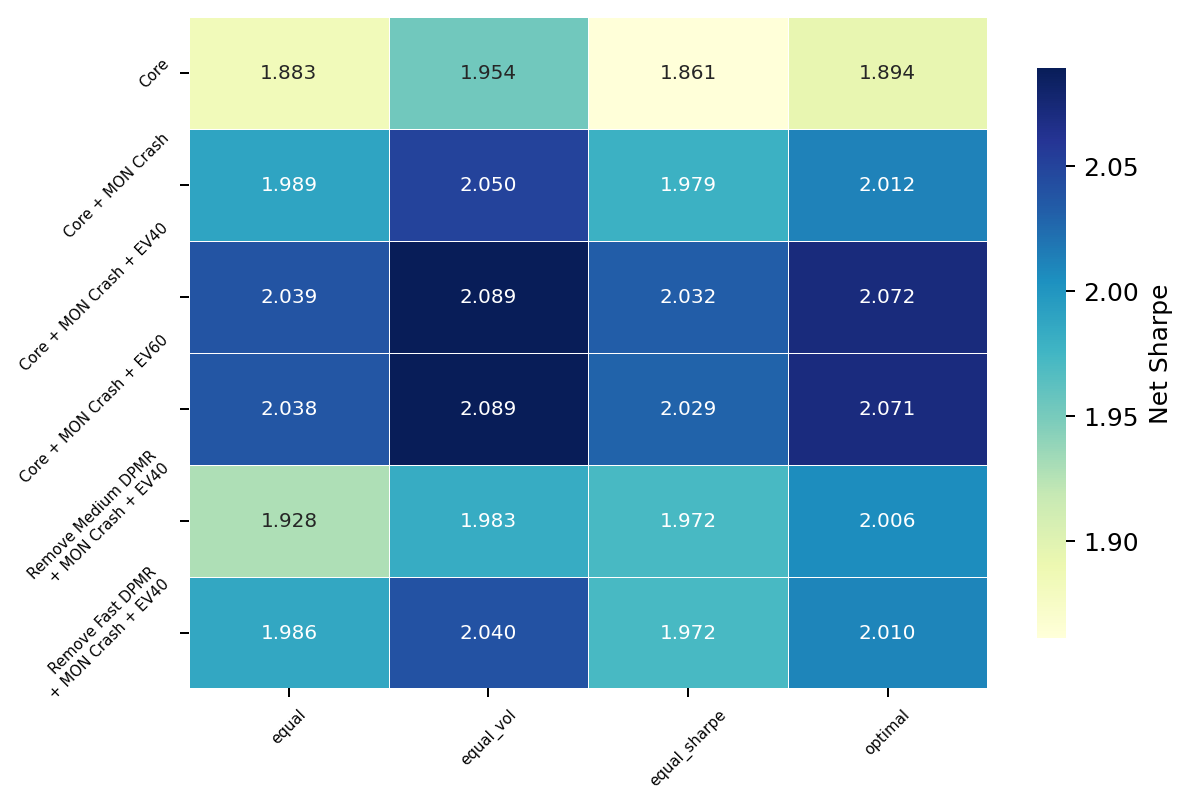
\includegraphics[width=0.75\textwidth]{figures/barbell_robustness_sharpe_heatmap.png}
    \caption{Sharpe ratio across extension variants and weighting schemes. The portfolio remains above 1.8 Sharpe across a wide range of configurations.}
    \label{fig:robustness}
\end{figure}

The portfolio was robust across weighting schemes. Equal-weight, equal-volatility, equal-Sharpe, and ridge-regularized mean-variance optimization all produced net Sharpes above 1.8. This is important because it indicates the diversification benefit is structural --- it doesn't depend on getting the weights exactly right.

Extension testing swept combinations of additional momentum, event-driven, and sector-relative sleeves. The best equal-weight extension paired one monotonic momentum sleeve with one residual-gap reversion sleeve, improving the base 6-sleeve portfolio from 1.883 to 2.039 Sharpe. But the key robustness finding is how stable the result was across nearby configurations:

\begin{itemize}
    \item \texttt{breadth\_40} vs \texttt{breadth\_60} gating on the event sleeve: 2.039 vs 2.038 Sharpe (effectively interchangeable)
    \item Adding a second event sleeve did not improve on the simpler two-sleeve extension
    \item Sector-relative sleeves helped as secondary diversifiers (1.972) but were not critical
\end{itemize}

Removing individual sleeves caused limited Sharpe degradation. No single sleeve removal dropped the portfolio below 1.8 Sharpe. This confirmed that the portfolio's strength comes from the diversification structure itself rather than from any one dominant alpha engine. The portfolio can tolerate the loss of any individual component without collapsing.

\subsection{Final Portfolio Attribution}

The attribution analysis of the final 8-sleeve equal-volatility portfolio shows how each component contributes to overall performance:

\begin{table}[htbp]
    \centering
    \small
    \begin{tabular}{lrrrrrr}
        \toprule
        Sleeve & Weight & Net SR & Ret.\ Contrib. & Var.\ Contrib. & Efficiency & Turn.\ Contrib. \\
        \midrule
        DPMR z60, always-on & 8.9\% & 1.549 & 16.1\% & 13.5\% & 1.189 & 23.0\% \\
        DPMR z60, vol expansion & 10.7\% & 1.394 & 14.4\% & 14.1\% & 1.025 & 17.0\% \\
        DPMR z20, vol contraction & 16.2\% & 1.336 & 13.8\% & 7.3\% & 1.900 & 13.0\% \\
        Residual MR (high resid.\ disp.) & 15.8\% & 1.192 & 12.3\% & 16.4\% & 0.751 & 4.9\% \\
        Resid.\ Gap Rev.\ (breadth) & 14.7\% & 1.177 & 12.2\% & 10.0\% & 1.224 & 28.5\% \\
        Active-Return MR (breadth) & 9.4\% & 1.098 & 11.4\% & 16.4\% & 0.693 & 3.3\% \\
        DPMR z10, panic & 15.8\% & 1.016 & 10.5\% & 13.0\% & 0.812 & 2.0\% \\
        Monotonic Momentum (crash) & 8.4\% & 0.888 & 9.2\% & 9.3\% & 0.986 & 8.3\% \\
        \bottomrule
    \end{tabular}
    \caption{Sleeve attribution for the final 8-sleeve equal-volatility portfolio.}
    \label{tab:sleeve-attribution}
\end{table}

Return contribution is spread evenly across sleeves --- the largest contributor accounts for 16.1\% and the smallest for 9.2\%, with most in the 10--14\% range. No single sleeve dominates. This is the attribution profile of a genuinely diversified portfolio, not a concentrated bet dressed up with peripheral hedges.

The vol-contraction DPMR sleeve is the most efficient component in the portfolio. It contributes 13.8\% of returns while accounting for only 7.3\% of variance --- an efficiency ratio of 1.9x. This sleeve acts as a stabilizing relative-value engine during calmer volatility regimes, adding return with relatively little incremental risk.

The residual gap-reversion sleeve is the most operationally expensive component (28.5\% of portfolio turnover) but contributes 12.2\% of returns with only 10\% of variance. It is expensive to trade, but it provides genuinely orthogonal alpha that justifies the cost. The residual MR and active-return MR sleeves occupy the opposite end of the spectrum --- they contribute moderate returns with low turnover (4.9\% and 3.3\%), functioning as stable core anchors rather than high-efficiency alpha generators.

During the portfolio's worst drawdown window (August 2021 to February 2022, 205 trading days), the panic DPMR sleeve and the monotonic momentum sleeve both experienced losses. Meanwhile, several core relative-value sleeves remained positive. This means the portfolio's drawdown resilience comes from structural diversification across sleeves rather than from any dedicated crash hedge --- the same correlation structure that justified the portfolio design in the first place is what protects it during stress.

\section{Implementation}

Some of the individual sleeves are turnover intensive, but the overall portfolio is substantially improved through diversification, conditioning, and slower horizon balancing. The final portfolio remains profitable under elevated transaction cost assumptions, has moderate aggregate turnover, and scales naturally through volatility targeting rather than raw directional exposure.

\subsection{Transaction Costs and Portfolio-Level Stabilization}

Several individual sleeves are fragile under higher cost assumptions. The residual gap-reversion sleeve (9.7\% daily turnover) drops from a 1.177 gross Sharpe to effectively zero at 20 bps and turns negative by 22 bps. The always-on DPMR sleeve (12.9\% daily turnover) degrades from a 1.549 gross Sharpe to 0.373 net at 25 bps. These are not robust standalone implementations.

The diversified portfolio tells a different story. At the baseline 10 bps assumption, the portfolio retains a 2.089 net Sharpe against a 2.611 gross --- a 20\% cost drag. At 16 bps, the portfolio still holds a 1.774 net Sharpe, while the residual gap sleeve has already dropped to 0.247 and the always-on DPMR to 0.794. At 25 bps --- roughly 2.5x a reasonable institutional estimate for liquid S\&P 500 names --- the portfolio retains a 1.304 Sharpe even as two of its eight sleeves have individually gone flat or negative.

\begin{figure}[htbp]
    \centering
    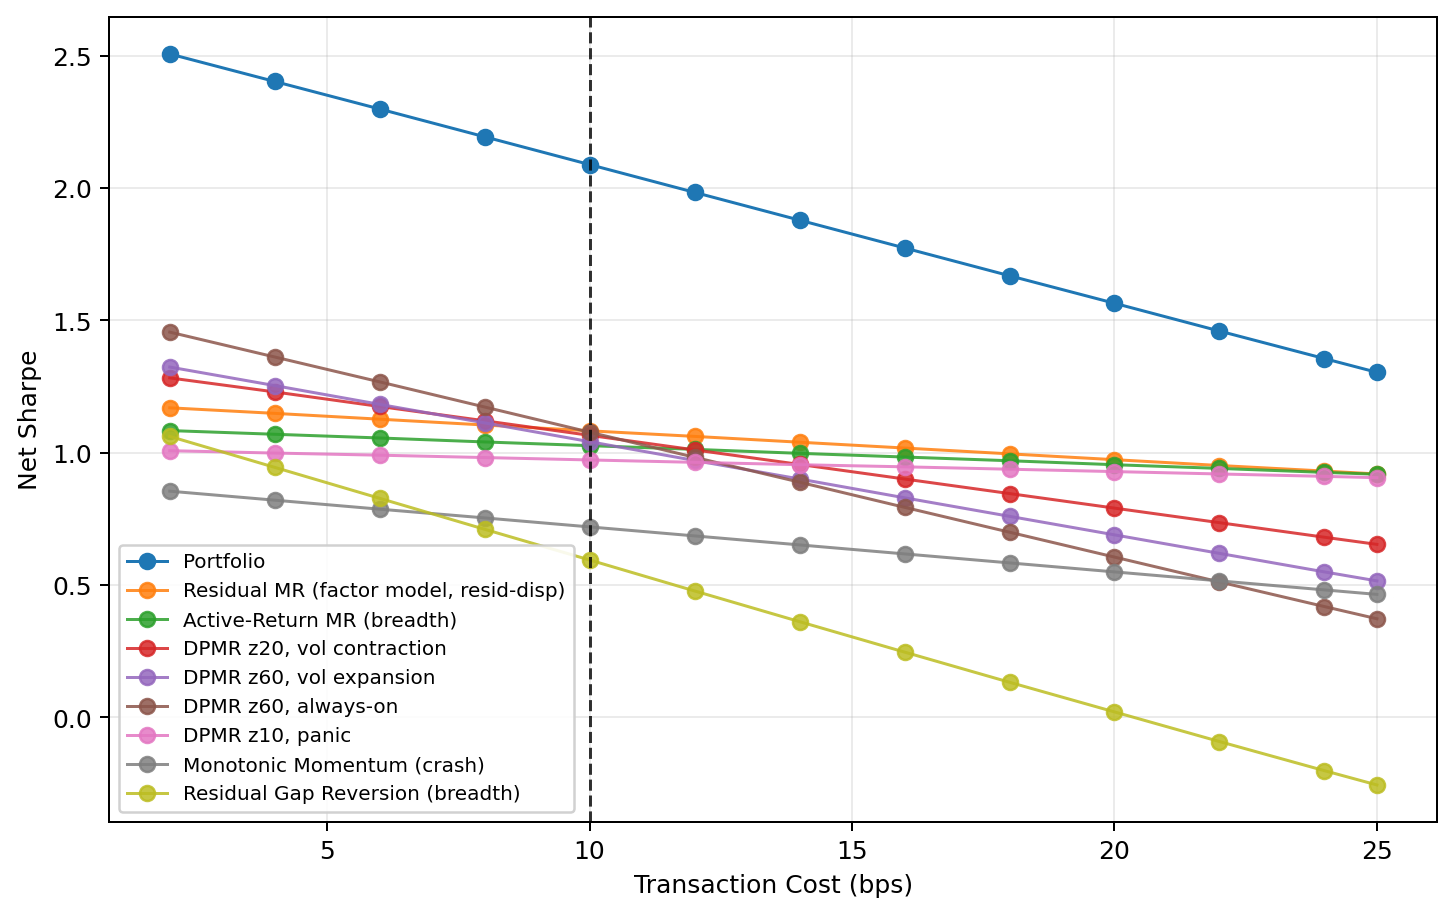
\includegraphics[width=0.75\textwidth]{figures/barbell_transaction_cost_sensitivity.png}
    \caption{Portfolio and sleeve-level net Sharpe across transaction cost assumptions from 2 to 25 bps.}
    \label{fig:cost-sensitivity}
\end{figure}

The portfolio's cost robustness comes from the same diversification structure that drives its Sharpe. High-turnover sleeves contribute alpha but their cost drag is diluted by lower-turnover sleeves that carry moderate but stable Sharpe ratios with minimal execution burden. The residual MR sleeve (1.5\% daily turnover) barely moves across cost assumptions --- 1.192 gross, 1.083 net at 10 bps, still 0.920 at 25 bps. The active-return MR sleeve behaves similarly. These stable core sleeves anchor the portfolio's cost profile while the faster sleeves contribute incremental alpha at lower cost levels.

\subsection{Turnover, Conditioning, and Capacity}

Aggregate portfolio turnover is 4.7\% daily --- moderate for a long-short portfolio --- but the execution burden is concentrated rather than evenly distributed across sleeves.

\begin{table}[htbp]
    \centering
    \small
    \begin{tabular}{lrll}
        \toprule
        Sleeve & Daily Turnover & Horizon & Capacity Notes \\
        \midrule
        \textbf{Portfolio (aggregate)} & \textbf{4.700\%} & \textbf{Multi-day} & \textbf{Moderate aggregate feasibility} \\
        DPMR z10 (panic) & 0.600\% & Episodic & Stressed windows only; low continuous burden \\
        Residual MR (resid.\ disp.) & 1.500\% & Medium & Easiest sleeve to scale \\
        Active-Return MR (breadth) & 1.800\% & Medium & Stable core sleeve \\
        DPMR z20 (vol contraction) & 4.000\% & Med-long & Monthly rebalance; requires crossing discipline \\
        Monotonic Momentum (crash) & 4.900\% & Med-long & Longer holding periods; cleaner execution \\
        DPMR z60 (vol expansion) & 8.000\% & Short-med & Faster rebalance; execution-dependent \\
        Resid.\ Gap Rev.\ (breadth) & 9.700\% & Short & Event-driven; trading quality matters \\
        DPMR z60 (always-on) & 12.900\% & Medium & Highest turnover; no conditioning filter \\
        \bottomrule
    \end{tabular}
    \caption{Turnover and capacity profile by sleeve.}
    \label{tab:turnover-capacity}
\end{table}

Conditioning plays a central role in making this turnover profile manageable. The conditioning framework does not just improve Sharpe --- it directly reduces implementation burden by keeping sleeves inactive during regimes where their signals are noisy and trades would be both alpha-poor and cost-expensive. The active-return MR sleeve illustrates this clearly: its base variant runs 11.7\% daily turnover with a 0.557 Sharpe, but after trend scaling and high residual-dispersion gating, turnover drops to 1.8\% while Sharpe rises to 1.279. The conditioning filter eliminated roughly 85\% of the trading activity while more than doubling risk-adjusted performance. Similar patterns appear in the residual MR sleeve (11.9\% $\rightarrow$ 1.5\% turnover), the sector-relative sleeve (11.9\% $\rightarrow$ 2.0\%), and the gap-reversion sleeve (11.1\% $\rightarrow$ 3.6\% after vol-contraction gating). Without conditioning, several of these sleeves would be operationally difficult and cost-prohibitive. With it, the slower residual MR and active-return MR sleeves become among the most scalable components in the portfolio.

The aggregate turnover remains moderate precisely because these conditioned low-turnover sleeves offset the faster distance-pairs and event-driven components. At moderate institutional scale, the portfolio's liquid large-cap universe (top-300 by rolling dollar volume) provides reasonable execution feasibility overall --- but the real execution burden and the binding capacity constraints are concentrated in the same three sleeves: the always-on DPMR (12.9\%), the residual gap-reversion (9.7\%), and the vol-expansion DPMR (8.0\%).

The always-on DPMR sleeve is the primary bottleneck. At 12.9\% daily turnover with no conditioning gate to reduce trade frequency, it generates continuous pair-spread trading activity across all market regimes. As capital scales, correlated positioning among pair-convergence traders would compress the spreads this sleeve trades, and execution slippage would compound with the already-high cost drag. The residual gap-reversion sleeve faces a different constraint: it concentrates trading immediately after large idiosyncratic moves, precisely when liquidity in the affected names is thinnest and bid-ask spreads are widest. The vol-expansion DPMR sleeve combines fast rebalancing (5-day) with activation during turbulent markets, when spread convergence is less reliable and slippage risk is elevated.

Live deployment at scale would require execution scheduling to avoid crossing against the same dislocations simultaneously across sleeves, borrow management for the short book, and dynamic participation controls to limit market impact in the fastest-rebalancing components. The slower residual MR and active-return MR sleeves would likely scale with minimal degradation; the fastest DPMR and event sleeves would be the first to encounter capacity limits.

\subsection{Leverage and Volatility Targeting}

Because the diversified portfolio maintains controlled drawdowns, low realized volatility ($\sim$2\% annualized unlevered), and stable cost characteristics after conditioning, leverage becomes a natural scaling mechanism rather than an independent enhancement. The portfolio behaves more like a diversified market-neutral risk-premia process than a high-volatility directional strategy, making volatility targeting a straightforward way to convert high risk-adjusted returns into economically meaningful absolute returns.

\begin{figure}[htbp]
    \centering
    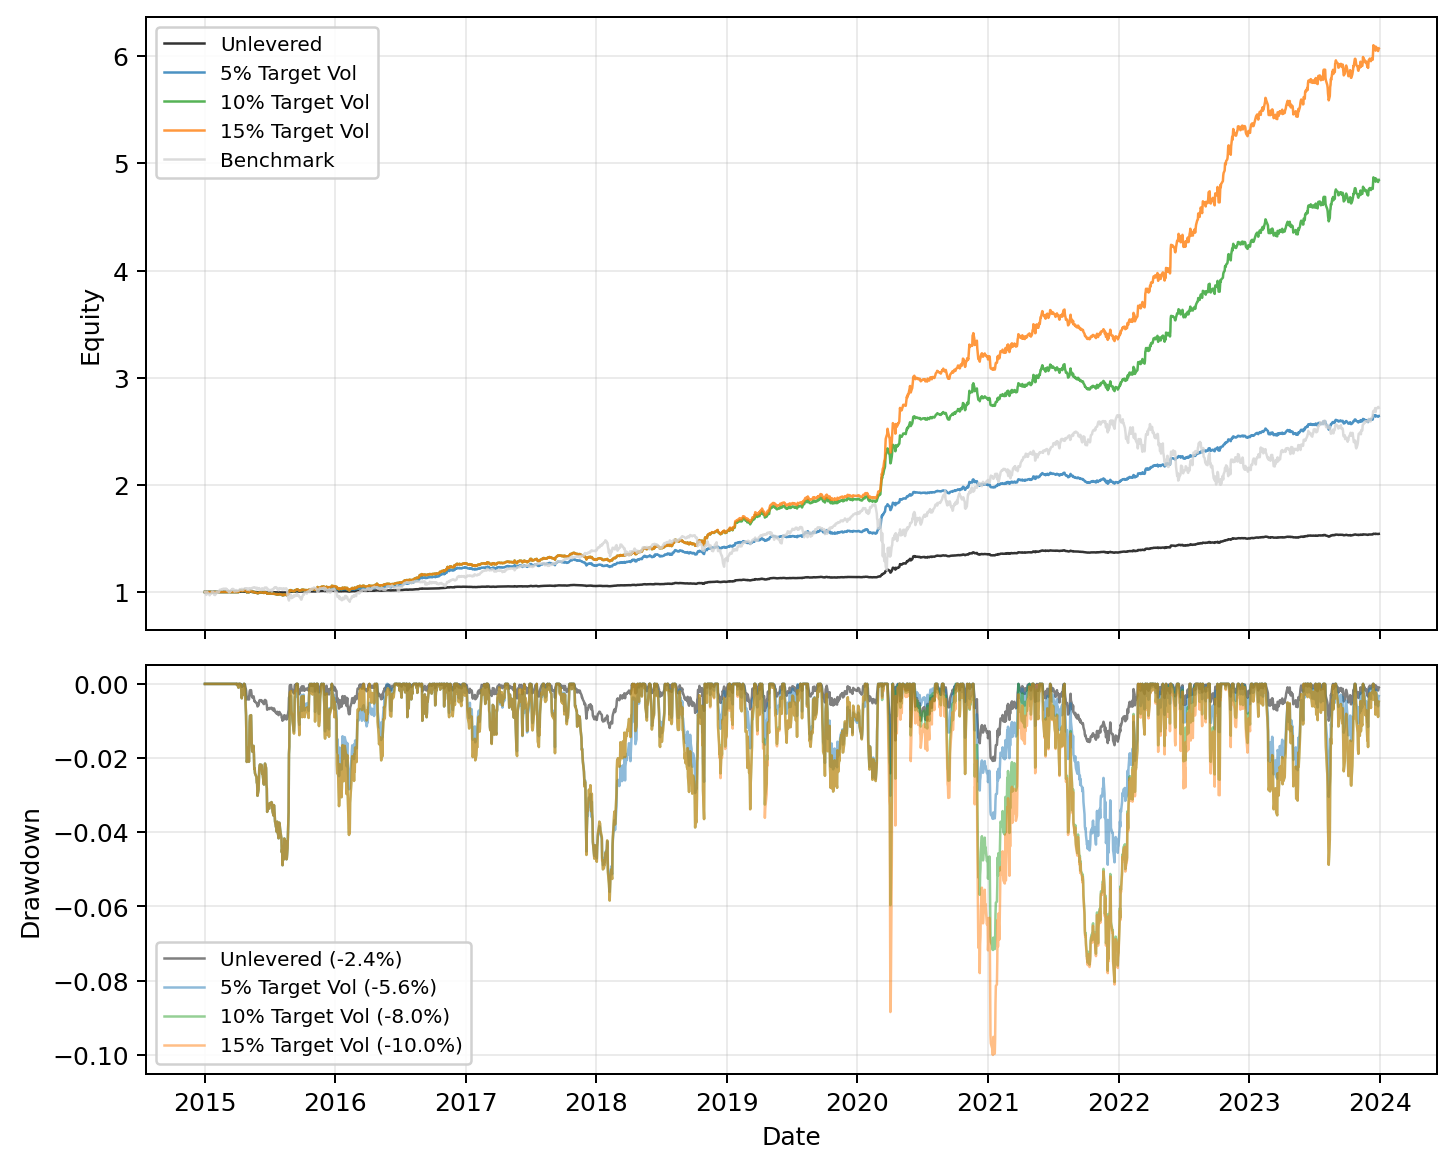
\includegraphics[width=0.75\textwidth]{figures/barbell_target_vol_equity_curves.png}
    \caption{Equity curves at different target volatility levels.}
    \label{fig:target-vol}
\end{figure}

Scaling to a 10\% target volatility substantially increases cumulative returns while maintaining moderate drawdowns. The levered series preserves the portfolio's structural properties --- sleeve correlations remain stable under leverage, conditioning and risk scaling continue functioning, and diversification between sleeves remains effective after scaling. Maximum drawdown on the levered series was roughly 14\%, and rolling Sharpe dynamics were stable rather than explosive. The leverage is feasible precisely because of the implementation characteristics described above: diversification across heterogeneous sleeves, conditioning-driven turnover reduction, and low cross-sleeve correlation produce a portfolio with the stability profile needed to support controlled leverage.

\section{Out-of-Sample Results}

The portfolio degraded out-of-sample but did not collapse. Post-2024, returns flattened, rolling Sharpe compressed, and drawdowns increased --- but the portfolio remained profitable, the equity curve continued trending upward, and diversification characteristics persisted. The trajectory suggests regime sensitivity rather than overfit failure.

\begin{figure}[htbp]
    \centering
    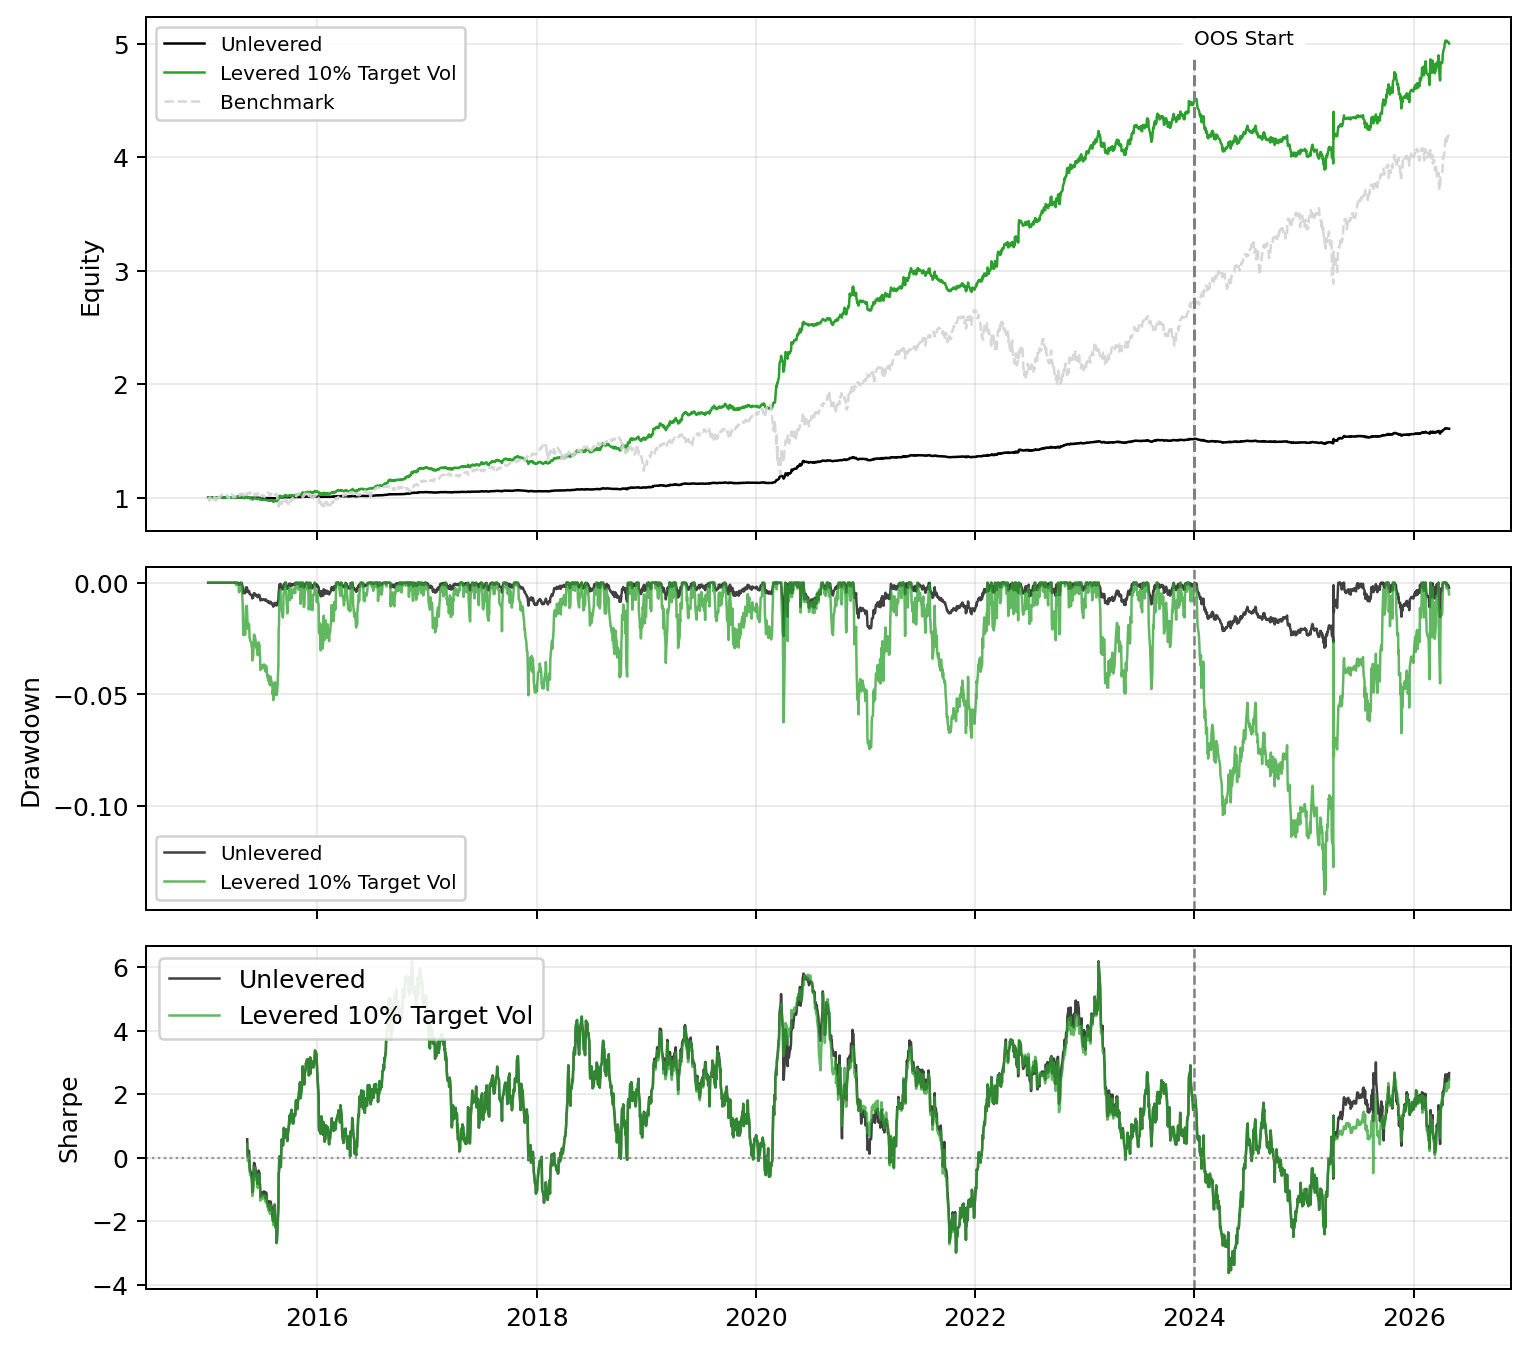
\includegraphics[width=0.75\textwidth]{figures/barbell_through_2026_04_summary.png}
    \caption{Portfolio equity curve from 2015 through April 2026, with the out-of-sample boundary at January 2024.}
    \label{fig:oos-equity}
\end{figure}

\begin{table}[htbp]
    \centering
    \small
    \begin{tabular}{clrrrrrrrr}
        \toprule
        Year & Period & Return & Sharpe & Vol & Max DD & Lev.\ Ret. & Lev.\ SR & Lev.\ Max DD & SPY Ret. \\
        \midrule
        2015 & IS & 1.100\% & 1.041 & 1.100\% & $-$1.100\% & 5.400\% & 1.010 & $-$5.300\% & 1.300\% \\
        2016 & IS & 3.800\% & 3.064 & 1.200\% & $-$0.400\% & 20.100\% & 3.064 & $-$2.100\% & 12.000\% \\
        2017 & IS & 0.500\% & 0.481 & 1.100\% & $-$1.000\% & 2.600\% & 0.481 & $-$5.100\% & 21.800\% \\
        2018 & IS & 3.200\% & 2.120 & 1.500\% & $-$0.900\% & 16.700\% & 2.116 & $-$4.200\% & $-$4.600\% \\
        2019 & IS & 3.900\% & 2.324 & 1.700\% & $-$0.700\% & 19.000\% & 2.251 & $-$3.600\% & 31.200\% \\
        2020 & IS & 18.300\% & 3.364 & 5.000\% & $-$2.400\% & 50.100\% & 3.235 & $-$6.300\% & 18.300\% \\
        2021 & IS & 1.300\% & 0.718 & 1.900\% & $-$1.400\% & 4.200\% & 0.528 & $-$7.000\% & 28.700\% \\
        2022 & IS & 9.000\% & 3.399 & 2.600\% & $-$0.600\% & 40.900\% & 3.388 & $-$2.600\% & $-$18.200\% \\
        2023 & IS & 2.400\% & 1.474 & 1.600\% & $-$1.000\% & 12.000\% & 1.466 & $-$5.000\% & 26.400\% \\
        \midrule
        \textbf{2024} & \textbf{OOS} & $\mathbf{-1.900\%}$ & $\mathbf{-1.350}$ & \textbf{1.400\%} & $\mathbf{-2.400\%}$ & $\mathbf{-9.200\%}$ & $\mathbf{-1.350}$ & $\mathbf{-11.400\%}$ & \textbf{24.900\%} \\
        \textbf{2025} & \textbf{OOS} & \textbf{4.900\%} & \textbf{1.273} & \textbf{3.800\%} & $\mathbf{-1.500\%}$ & \textbf{12.800\%} & \textbf{0.840} & $\mathbf{-6.700\%}$ & \textbf{17.900\%} \\
        \textbf{2026} & \textbf{OOS} & \textbf{9.900\%} & \textbf{2.414} & \textbf{4.000\%} & $\mathbf{-1.500\%}$ & \textbf{31.500\%} & \textbf{2.136} & $\mathbf{-4.500\%}$ & \textbf{15.100\%} \\
        \bottomrule
    \end{tabular}
    \caption{Annual performance summary. IS = in-sample (2015--2023), OOS = out-of-sample (2024--2026). Lev.\ columns reflect 10\% target volatility scaling.}
    \label{tab:annual-performance}
\end{table}

2024 is the only negative-return year in the entire series ($-$1.9\% unlevered, $-$1.350 Sharpe), and the evidence points to regime instability rather than structural decay. Strong index trends and concentrated mega-cap leadership reduced cross-sectional reversal opportunities. Momentum persistence was unfavorable to the portfolio's predominantly mean-reversion construction. Reduced idiosyncratic dispersion weakened the signals that depend on cross-sectional spread. A portfolio built on short-horizon mean reversion, statistical arbitrage, and relative-value convergence should struggle in exactly this kind of environment. The fact that it did is economically consistent with the portfolio design.

The recovery after 2024 is important for distinguishing regime sensitivity from overfit. Rather than continuing to decay --- which would suggest structural overfit --- the portfolio recovered in 2025 (1.273 Sharpe, +4.9\%) and strengthened further in 2026 through April (2.414 Sharpe, +9.9\%). This trajectory --- drawdown, recovery, resumed positive performance --- supports the interpretation that the weakness was temporary regime-driven degradation rather than a dead strategy. The portfolio performs best during high-dispersion environments: 2020 (COVID volatility, 3.364 Sharpe) and 2022 (rate-driven selloff, 3.399 Sharpe) were the standout years by a wide margin. In these periods, cross-sectional opportunity expands as more stocks move independently, the crisis-conditioned DPMR and event sleeves engage specifically during high-volatility episodes, and several volatility-gated sleeves activate during vol expansion.

Beyond point Sharpe estimates, the portfolio retained its structural diversification properties throughout the out-of-sample period. Benchmark correlation remained low, drawdowns stayed materially smaller than SPY's, and volatility remained controlled. These characteristics persisted across the regime shift. The levered 10\% target-vol series produced 12--20\% returns in favorable environments, $-$9.2\% in the worst OOS year (2024), and a maximum drawdown of $-$11.4\%. The 50.1\% return in 2020 reflects stat-arb dispersion exploding during COVID --- extreme but economically consistent. Rolling Sharpe dynamics remained stable rather than explosive under leverage, confirming that diversification between sleeves remained effective after scaling and that conditioning continued functioning out-of-sample.

The out-of-sample results do not show that this portfolio works equally well in all environments --- nor should they. They do show persistence of edge, robustness of the diversification structure, and continued positive expectancy after unseen data exposure. The portfolio is regime-dependent, and the OOS period demonstrated both the cost of that dependence (2024) and the benefit of structural resilience (2025--2026 recovery).

\section{Risks}

Several important limitations and risks remain despite the portfolio's strong in-sample and out-of-sample performance.

The largest methodological risk is overfitting. The research process explored a broad space of signal families, conditioning filters, rebalance schedules, scaling rules, and portfolio combinations. Although the workflow emphasized economic intuition and robustness rather than aggressive parameter optimization --- and the later out-of-sample period provides a genuine holdout test --- repeated experimentation inevitably increases the probability that some results reflect noise rather than persistent structure.

The dataset itself also introduces uncertainty. Data was sourced through yfinance, which does not guarantee a survivorship-bias-free historical universe. Historical S\&P 500 membership may therefore be imperfectly reconstructed, potentially overstating results by excluding delisted or distressed securities that would have existed in a true historical universe.

The portfolio is also regime-dependent. Most sleeves are fundamentally relative-value or mean-reversion strategies, which can struggle during persistent directional trends, momentum-driven markets, or structural dislocations where convergence relationships temporarily break down. This behavior was visible during the 2024 out-of-sample period, where the portfolio experienced its weakest sustained performance during a strong momentum regime before recovering later in the sample. The monotonic momentum sleeve partially offsets this exposure, but the portfolio still retains a structural bias toward cross-sectional convergence behavior.

Implementation and market structure risks are also meaningful. Several sleeves --- particularly the always-on distance-pairs sleeve and the residual gap-reversion sleeve --- are sensitive to transaction costs, slippage, and execution quality. The constant 10 bps transaction cost assumption is a simplification and may understate costs during stressed or crowded conditions. As capital scales, crowding effects, borrow constraints, spread widening, or execution delays could materially reduce realized performance.

Finally, the portfolio's diversification properties may not remain stable over time. Much of the portfolio strength comes from combining sleeves with low realized correlation and different regime sensitivities. If market structure changes cause these alpha streams to become more correlated --- for example through increased statistical arbitrage crowding or homogenization of systematic strategies --- then portfolio-level Sharpe could deteriorate even if individual sleeves remain independently profitable.

\section{Conclusion}

The final eight-sleeve portfolio achieved a 2.039 net Sharpe ratio after 10 basis points of transaction costs in-sample, with no single sleeve contributing more than 16\% of returns. The portfolio's strength came from diversification across economically distinct alpha sources --- distance-pairs relative value as the orthogonal structural core, conditioned mean-reversion variants as stable low-turnover anchors, and monotonic momentum and gap reversion as regime-complementary diversifiers. Conditioning filters improved implementation quality primarily by reducing turnover rather than increasing gross alpha, transforming several otherwise cost-prohibitive sleeves into scalable portfolio components. The diversification structure proved robust: equal-weight, equal-volatility, and optimized weighting schemes all produced net Sharpes above 1.8, ablation of any single sleeve caused limited degradation, and the portfolio retained a 1.304 Sharpe even at 25 bps of assumed costs.

Out-of-sample, the portfolio degraded during the momentum-dominated regime of 2024 ($-$1.9\% return, $-$1.350 Sharpe) but recovered in 2025 and strengthened through April 2026 (2.414 Sharpe), consistent with regime sensitivity rather than overfit. Benchmark correlation remained low and drawdowns stayed controlled throughout. The results suggest that diversification across heterogeneous signal families --- rather than selection of individually optimal signals --- is the more reliable path to stable portfolio-level performance in cross-sectional equity strategies. Natural extensions include walk-forward optimization for parameter stability testing, dynamic regime-aware sleeve weighting, more realistic execution and market impact modeling, and expansion beyond the S\&P 500 universe.

\end{document}
